%--------------------
% Packages
% -------------------
\documentclass[12pt,a4paper]{article}
\usepackage[utf8x]{inputenc}
\usepackage[T1]{fontenc}
%\usepackage{gentium}
\usepackage{mathptmx} % Use Times Font


\usepackage[pdftex]{graphicx} % Required for including pictures
\usepackage[swedish]{babel} % Swedish translations
\usepackage[pdftex,linkcolor=black,pdfborder={0 0 0}]{hyperref} % Format links for pdf
\usepackage{calc} % To reset the counter in the document after title page
\usepackage{enumitem} % Includes lists

\frenchspacing % No double spacing between sentences
\linespread{1.2} % Set linespace
\usepackage[a4paper, lmargin=0.1666\paperwidth, rmargin=0.1666\paperwidth, tmargin=0.1111\paperheight, bmargin=0.1111\paperheight]{geometry} %margins
%\usepackage{parskip}

\usepackage[all]{nowidow} % Tries to remove widows
\usepackage[protrusion=true,expansion=true]{microtype} % Improves typography, load after fontpackage is selected

\usepackage{xcolor}
\usepackage{hyperref}
\hypersetup{
    colorlinks=true,
    linkcolor=blue,      
    urlcolor=cyan,
}

%-----------------------
% Set pdf information and add title, fill in the fields
%-----------------------
\hypersetup{ 	
pdfsubject = {IPK},
pdftitle = {Sniffer},
pdfauthor = {Pavel Yadlouski}
}

%-----------------------
% Begin document
%-----------------------
\title{Project IPK \\
Sniffer}

\author{Pavel Yadlouski (xyadlo00)}
\begin{document}

\begin{titlepage}
   \begin{center}
       \vspace*{1cm}
       \Large{ 
           \begin{figure}
               \centering
               
\includegraphics[width=\textwidth,height=\textheight,keepaspectratio]{VUT-FIT-logo-en.png}
           \end{figure}

           \textbf{Project IPK\\Sniffer}
           
           \vspace{0.5cm}
           Variant ZETA
           
           \vspace{1.5cm}
           
           \textbf{Pavel Yadlouski (xyadlo00)}
           
           \vfill
        }
           
           
           \vspace{0.8cm}
     
       Brno University of Technologies\\
       April, 2020
            
   \end{center}
\end{titlepage}

\section*{Introduction}

This documentation for school project on Brno University of Technologies. Aim of 
the project is to implement packet sniffer. Project is implemented in C language 
using library \textit{libpcap}\footnote{\url{https://www.tcpdump.org/manpages/pcap.3pcap.html}}.
Also for understanding concepts of building programs with   \textit{libpcap}, 
tutorial\footnote{\url{https://www.tcpdump.org/pcap.html}} from official web 
site was used.
\section{Architecture of program}

Main function is presented in file \texttt{sniffer.c}. This function should 
parse input parameters, check if this parameters are correct. In case of 
parameter \textit{-h (-{}-help)} write down basic information about program. 
Also writing information about program is default behavior when any parameter is 
set. 

After parsing parameters and setting corresponding flags, then given device 
should be open for sniffing. Also on this step filter should be made. If there 
are no parameters for creating filter, then default filter would be used, that 
means sniffer would process TCP \textbf{and} UDP packets on \textbf{any} port. 

Finally device is putted in loop for processing input packets. Process packet 
means extract necessary information from packet headers and after that print out 
whole packet. Format of printing out is:
\begin{verbatim}
    time source_address: port -> destination_address: port
    count_of_printed_bytes: bytes_in_hex bytes_in_ASCII
\end{verbatim}    


\section{Implementation details}

Program is separated into two files: \texttt{sniffer.c} and \texttt{function.c}. 
As was mentioned, first file contain \textit{main} function. In this function 
parameters are parsed in \textit{while} loop using \texttt{getopt\_long} function. 
This function returns to local variable parameters one by one. Then follows  
\textit{switch case}, where value of parameter is set to corresponding global 
variable. This global variables are defined in second file -- \texttt{function.c}. 

Preparations for sniffing given device are held in function \textit{start\_loop}, 
that follows after parameters parsing. This function defined in file 
\texttt{functions.c}. There is opening interface for sniffing as first step of 
preparations. If given interface is not valid, then corresponding error would 
appear. After that creating of filter follows. Filtering options are constructed 
in function \textit{create\_filter} which creates string with filter parameters. 
As specified in \textit{libpcap} documentation, filter is set using function 
\textit{pcap\_compile} followed be function \textit{pcap\_setfilter}. 

After setting filter processing loop follows. In this loop each packet is 
captured by \textit{pcap\_next} function. Then packet passed to function that 
make actual processing of packet -- \textit{process\_packet}. Processing of 
packet is made based on type of packet: UDP or TCP. This information is used for 
extracting valid header and get from there valid source and destination ports. 
After that printing of packet follows. 

As first, timestamp is converted to human-readable format with microsecond. 
Then source address and port are printed out followed by destination address and 
port. Packet is hexadecimal format is printed out in maximum 16 bytes per line 
and followed by ASCII representation of printed bytes. 

For correct printing of packet there is function \textit{print\_data}. In this 
function there is loop which goes with step of maximum value of bytes. By 
default, this maximum value is set to 16 In the beginning of each line there is 
last offset from the beginning of packet of cursor in hexadecimal format. Also 
this number gives number of already printed bytes. In this loop there one more 
loop for printing byte by byte that goes from current offset to next 16 bytes. 
End of packet is detected by following statement:
\begin{verbatim}
    if (current_offset + 16 >= size_of_packet){
        maximum_value = size_of_packet - current_offset;
    }
\end{verbatim}

\section{Testing}

Testing of program was made comparing printed result with captured packets by 
program \texttt{Wireshark}\footnote{\url{https://www.wireshark.org/}} 

Fore testing purpose sniffer was executed with following command
\begin{verbatim}
    sudo ./ipk-sniffer -i wlp2s0 --tcp -p 443 -n 2 
\end{verbatim}
which set sniffer to sniff interface \textit{wlp2s0}, filter only tcp packet on 
port 443 and end sniffing after two packet was captured. For Wireshark capturing 
filter was set like 
\begin{verbatim}
    tcp port 443
\end{verbatim} 
on interface \textit{wlp2s0}

Here you can see screenshots from Wireshark compering with output of my program:

\begin{figure}[h!]
    \centering
    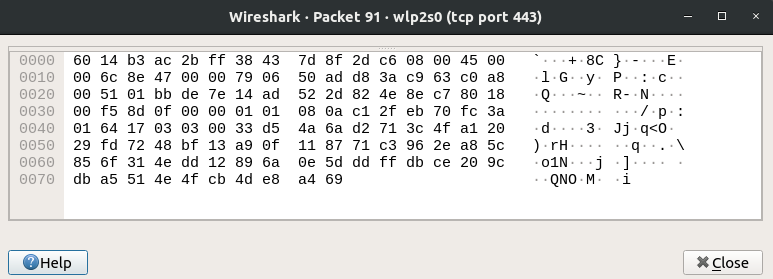
\includegraphics[width=\textwidth,height=\textheight,keepaspectratio]{first_packet.png}
    \caption{First packet captured by Wireshark}
\end{figure}

\begin{figure}[h!]
    \centering
    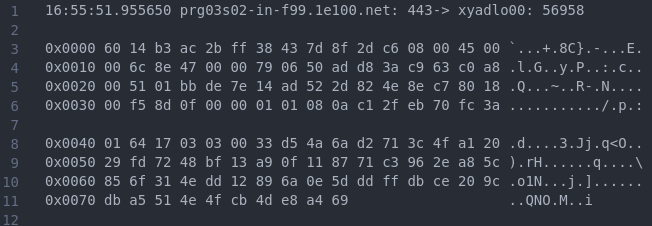
\includegraphics[width=\textwidth,height=\textheight,keepaspectratio]{my_first_packet.png}
    \caption{First packet captured by sniffer}
\end{figure}

\begin{figure}[h!]
    \centering
    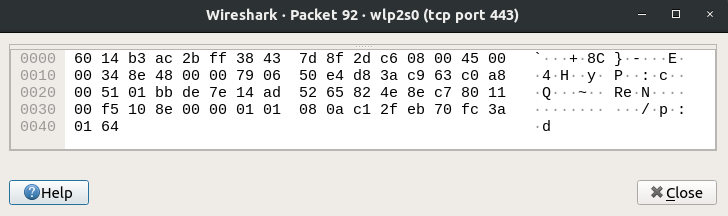
\includegraphics[width=\textwidth,height=\textheight,keepaspectratio]{second_packet.png}
    \caption{Second packet captured by Wireshark}
\end{figure}

\begin{figure}[h!]
    \centering
    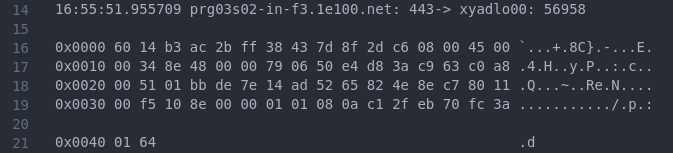
\includegraphics[width=\textwidth,height=\textheight,keepaspectratio]{my_second_packet.png}
    \caption{Second packet captured by sniffer}
\end{figure}


\end{document}
